\documentclass[10pt,a4paper]{article}
\usepackage[utf8]{inputenc}
\usepackage[top=2cm,bottom=2cm,left=2cm,right=2cm]{geometry}
\usepackage{amsmath}
\usepackage{amssymb}
\usepackage{array}
\usepackage{tikz}
\usetikzlibrary{arrows.meta,calc,patterns,positioning}
\usepackage{pgfplots}
\pgfplotsset{compat=1.18}
\usepackage[dvipsnames,svgnames]{xcolor}
\usepackage{hyperref}

% Anchor persamaan unik meski nomor di-reset per soal.
\newcounter{eqblock}
\newcommand{\reseteq}{%
  \stepcounter{eqblock}%
  \setcounter{equation}{0}%
  \renewcommand{\theHequation}{\arabic{eqblock}.\arabic{equation}}%
}

\pgfplotsset{
  grafik/.style={
    axis lines=middle,
    xlabel={$x$}, ylabel={$y$},
    width=7.5cm, height=6cm,
    grid=major, grid style={gray!25},
    tick label style={font=\scriptsize},
    every axis x label/.style={at={(ticklabel* cs:1)},anchor=west},
    every axis y label/.style={at={(ticklabel* cs:1)},anchor=south},
    title style={yshift=2ex},
  },
}

\title{Tugas Minggu 10 : Fungsi Transenden}
\author{Matematika untuk Sistem Informasi}
\date{}

\begin{document}

\maketitle

\begin{enumerate}

%===========================================================
\item Tentukan turunan pertama dari fungsi berikut.
\begin{enumerate}

%-----------------------------------------------------------
\item $\displaystyle f(x) = \ln\left(\frac{1 + x}{1 - x}\right)$

\textbf{Jawab:}
\begin{itemize}
\item \textbf{Langkah 1: Tentukan Domain}

Logaritma memerlukan $\frac{1 + x}{1 - x} > 0$, yang dipenuhi tepat untuk $-1 < x < 1$. Pada selang ini $1 + x > 0$ dan $1 - x > 0$.

\item \textbf{Langkah 2: Uraikan dengan Sifat Logaritma (Cara 1)}

Hasil bagi di dalam $\ln$ dipecah menjadi selisih, lalu setiap suku diturunkan:
\reseteq
\begin{align}
f(x) &= \ln(1 + x) - \ln(1 - x) \quad \text{(Sifat hasil bagi)} \\
f'(x) &= \frac{1}{1 + x} - \frac{-1}{1 - x} = \frac{1}{1 + x} + \frac{1}{1 - x} \\
&= \frac{(1 - x) + (1 + x)}{(1 + x)(1 - x)} = \frac{2}{1 - x^2}
\end{align}

\item \textbf{Langkah 3: Cek dengan Rumus $\frac{u'}{u}$ (Cara 2)}

Dengan $u = \frac{1 + x}{1 - x}$, aturan hasil bagi memberi
\reseteq
\begin{align}
u'(x) &= \frac{(1 - x) \cdot 1 - (1 + x) \cdot (-1)}{(1 - x)^2} = \frac{2}{(1 - x)^2} \\
f'(x) &= \frac{u'}{u} = \frac{2}{(1 - x)^2} \cdot \frac{1 - x}{1 + x} = \frac{2}{(1 - x)(1 + x)} = \frac{2}{1 - x^2}
\end{align}
Kedua cara memberikan hasil yang sama.
% final: f'(x) = \frac{2}{1 - x^2}
\end{itemize}

%-----------------------------------------------------------
\item $f(x) = \ln(\tan 2x)$

\textbf{Jawab:}
\begin{itemize}
\item \textbf{Langkah 1: Tentukan $u$ dan $u'$}

Misalkan $u = \tan 2x$ (dengan $\tan 2x > 0$), maka $u' = 2\sec^2 2x$.

\item \textbf{Langkah 2: Gunakan Rumus $\frac{u'}{u}$ dan Sederhanakan}

Tulis $\sec$ dan $\tan$ dalam $\sin$ dan $\cos$:
\reseteq
\begin{align}
f'(x) &= \frac{2\sec^2 2x}{\tan 2x} = \frac{2}{\cos^2 2x} \cdot \frac{\cos 2x}{\sin 2x} = \frac{2}{\sin 2x\cos 2x} \\
&= \frac{4}{2\sin 2x\cos 2x} = \frac{4}{\sin 4x} \quad \text{(Sudut ganda: $2\sin\theta\cos\theta = \sin 2\theta$)} \\
&= 4\csc 4x
\end{align}
% final: f'(x) = 4\csc 4x
\end{itemize}

%-----------------------------------------------------------
\item $f(x) = \ln(x^2 - 5x + 6)$

\textbf{Jawab:}
\begin{itemize}
\item \textbf{Langkah 1: Tentukan Domain}

$x^2 - 5x + 6 = (x - 2)(x - 3) > 0$ untuk $x < 2$ atau $x > 3$.

\item \textbf{Langkah 2: Gunakan Rumus $\frac{u'}{u}$}

Dengan $u = x^2 - 5x + 6$ dan $u' = 2x - 5$ (sama dengan Contoh~3.2(b) pada Topik~8):
\reseteq
\begin{align}
f'(x) &= \frac{2x - 5}{x^2 - 5x + 6}
\end{align}
% final: f'(x) = \frac{2x - 5}{x^2 - 5x + 6}
\end{itemize}

%-----------------------------------------------------------
\item $f(x) = \ln(x^3 + 3x)$

\textbf{Jawab:}
\begin{itemize}
\item \textbf{Langkah 1: Tentukan Domain}

$x^3 + 3x = x(x^2 + 3) > 0$ untuk $x > 0$, karena $x^2 + 3 > 0$.

\item \textbf{Langkah 2: Gunakan Rumus $\frac{u'}{u}$}

Dengan $u = x^3 + 3x$ dan $u' = 3x^2 + 3$:
\reseteq
\begin{align}
f'(x) &= \frac{3x^2 + 3}{x^3 + 3x} = \frac{3(x^2 + 1)}{x(x^2 + 3)}
\end{align}
% final: f'(x) = \frac{3(x^2 + 1)}{x(x^2 + 3)}
\end{itemize}

%-----------------------------------------------------------
\item $f(x) = \sin\bigl(\ln(2x + 1)\bigr)$

\textbf{Jawab:}
\begin{itemize}
\item \textbf{Langkah 1: Fungsi Dalam}

Misalkan $u = \ln(2x + 1)$ (dengan $x > -\frac{1}{2}$), maka $u' = \frac{2}{2x + 1}$.

\item \textbf{Langkah 2: Aturan Rantai}

Lapisan luar $\sin u$ diturunkan menjadi $\cos u$ (sama dengan Latihan Mandiri~6.1 no.~4 pada Topik~8):
\reseteq
\begin{align}
f'(x) &= \cos\bigl(\ln(2x + 1)\bigr) \cdot \frac{2}{2x + 1} = \frac{2\cos\bigl(\ln(2x + 1)\bigr)}{2x + 1}
\end{align}
% final: f'(x) = \frac{2\cos(\ln(2x + 1))}{2x + 1}
\end{itemize}

%-----------------------------------------------------------
\item $f(x) = x^5 e^{2x^2}$

\textbf{Jawab:}
\begin{itemize}
\item \textbf{Langkah 1: Turunan Setiap Faktor}

$u = x^5$ memberi $u' = 5x^4$. $v = e^{2x^2}$ memberi $v' = e^{2x^2} \cdot 4x = 4x\, e^{2x^2}$ (aturan rantai).

\item \textbf{Langkah 2: Aturan Hasil Kali $(uv)' = u'v + uv'$}

Gabungkan kedua turunan faktor:
\reseteq
\begin{align}
f'(x) &= 5x^4 e^{2x^2} + x^5 \cdot 4x\, e^{2x^2} = 5x^4 e^{2x^2} + 4x^6 e^{2x^2} \\
&= x^4(5 + 4x^2)\, e^{2x^2} \quad \text{(Faktorkan $x^4 e^{2x^2}$)}
\end{align}
% final: f'(x) = x^4(5 + 4x^2) e^{2x^2}
\end{itemize}

\end{enumerate}

%===========================================================
\item Tentukan hasil integral berikut.
\begin{enumerate}

%-----------------------------------------------------------
\item $\displaystyle\int \frac{4}{2x + 1}\, dx$

\textbf{Jawab:}
\begin{itemize}
\item \textbf{Langkah 1: Pilih $u$}

Misalkan $u = 2x + 1$, maka $du = 2\, dx$, sehingga $dx = \frac{1}{2}\, du$.

\item \textbf{Langkah 2: Substitusi dan Integralkan}

Sama dengan Contoh~3.3(a) pada Topik~8:
\reseteq
\begin{align}
\int \frac{4}{2x + 1}\, dx &= 4 \cdot \frac{1}{2}\int \frac{1}{u}\, du = 2\ln|u| + C = 2\ln|2x + 1| + C
\end{align}
% final: 2\ln|2x + 1| + C
\end{itemize}

%-----------------------------------------------------------
\item $\displaystyle\int \frac{4x + 2}{x^2 + x + 5}\, dx$

\textbf{Jawab:}
\begin{itemize}
\item \textbf{Langkah 1: Pembilang Kelipatan Turunan Penyebut}

Misalkan $u = x^2 + x + 5$, maka $du = (2x + 1)\, dx$, dan $4x + 2 = 2(2x + 1)$.

\item \textbf{Langkah 2: Substitusi dan Integralkan}

Pembilang menjadi $2\, du$:
\reseteq
\begin{align}
\int \frac{4x + 2}{x^2 + x + 5}\, dx &= 2\int \frac{1}{u}\, du = 2\ln|x^2 + x + 5| + C = 2\ln(x^2 + x + 5) + C
\end{align}
Tanda mutlak boleh dilepas karena $x^2 + x + 5 = \left(x + \frac{1}{2}\right)^2 + \frac{19}{4} > 0$ untuk setiap $x$.
% final: 2\ln(x^2 + x + 5) + C
\end{itemize}

%-----------------------------------------------------------
\item $\displaystyle\int \frac{\sin(\ln x)}{x}\, dx$

\textbf{Jawab:}
\begin{itemize}
\item \textbf{Langkah 1: Pilih $u$}

Misalkan $u = \ln x$, maka $du = \frac{1}{x}\, dx$.

\item \textbf{Langkah 2: Substitusi dan Integralkan}

Faktor $\frac{1}{x}\, dx$ diganti dengan $du$:
\reseteq
\begin{align}
\int \sin(\ln x) \cdot \frac{1}{x}\, dx &= \int \sin u\, du = -\cos u + C = -\cos(\ln x) + C
\end{align}
% final: -\cos(\ln x) + C
\end{itemize}

%-----------------------------------------------------------
\item $\displaystyle\int (x + 3)e^{x^2 + 6x}\, dx$

\textbf{Jawab:}
\begin{itemize}
\item \textbf{Langkah 1: Pilih $u$ dan Sesuaikan Konstanta}

Misalkan $u = x^2 + 6x$, maka $du = (2x + 6)\, dx = 2(x + 3)\, dx$, sehingga $(x + 3)\, dx = \frac{1}{2}\, du$.

\item \textbf{Langkah 2: Substitusi dan Integralkan}

Sama dengan Contoh~5.4(g) pada Topik~8:
\reseteq
\begin{align}
\int (x + 3)e^{x^2 + 6x}\, dx &= \frac{1}{2}\int e^u\, du = \frac{1}{2}e^u + C = \frac{1}{2}e^{x^2 + 6x} + C
\end{align}
% final: \frac{1}{2}e^{x^2 + 6x} + C
\end{itemize}

%-----------------------------------------------------------
\item $\displaystyle\int (\cos x)\, e^{\sin x}\, dx$

\textbf{Jawab:}
\begin{itemize}
\item \textbf{Langkah 1: Pilih $u$}

Misalkan $u = \sin x$, maka $du = \cos x\, dx$.

\item \textbf{Langkah 2: Substitusi dan Integralkan}

Faktor $\cos x\, dx$ diganti dengan $du$:
\reseteq
\begin{align}
\int (\cos x)\, e^{\sin x}\, dx &= \int e^u\, du = e^u + C = e^{\sin x} + C
\end{align}
% final: e^{\sin x} + C
\end{itemize}

%-----------------------------------------------------------
\item $\displaystyle\int_0^4 \frac{x^2}{x^3 + 2}\, dx$

\textbf{Jawab:}
\begin{itemize}
\item \textbf{Langkah 1: Pilih $u$ dan Sesuaikan Konstanta}

Misalkan $u = x^3 + 2$, maka $du = 3x^2\, dx$, sehingga $x^2\, dx = \frac{1}{3}\, du$.

\item \textbf{Langkah 2: Ubah Batas}

Untuk $x = 0$ diperoleh $u = 2$, dan untuk $x = 4$ diperoleh $u = 64 + 2 = 66$.

\item \textbf{Langkah 3: Substitusi dan Hitung}

Gunakan $\int \frac{1}{u}\, du = \ln|u|$ dan Teorema Dasar Kalkulus II:
\reseteq
\begin{align}
\int_0^4 \frac{x^2}{x^3 + 2}\, dx &= \frac{1}{3}\int_2^{66} \frac{1}{u}\, du = \frac{1}{3}\Bigl[\ln|u|\Bigr]_2^{66} = \frac{1}{3}(\ln 66 - \ln 2) \\
&= \frac{1}{3}\ln\frac{66}{2} = \frac{1}{3}\ln 33 \approx 1{,}1655 \quad \text{(Sifat hasil bagi)}
\end{align}

\item \textbf{Langkah 4: Tafsiran Geometri}

Karena $\frac{x^2}{x^3 + 2} \ge 0$ pada $[0, 4]$, nilai integral sama dengan luas daerah di bawah kurva:

\begin{center}
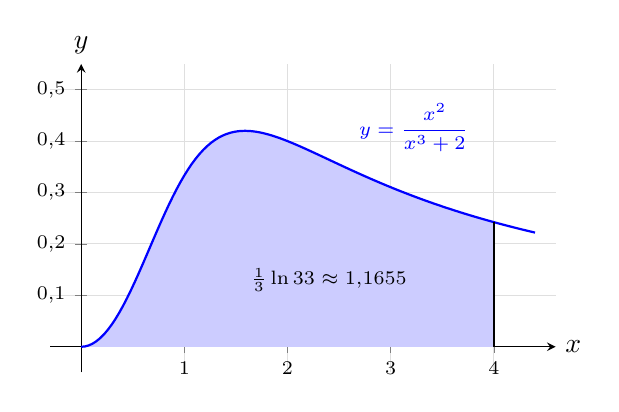
\begin{tikzpicture}
\begin{axis}[grafik, width=8cm, height=5.5cm, xmin=-0.3, xmax=4.6, ymin=-0.05, ymax=0.55, xtick={1,2,3,4}, ytick={0.1,0.2,0.3,0.4,0.5}, yticklabel style={/pgf/number format/use comma}]
  \addplot[domain=0:4, samples=100, fill=blue!20, draw=none] {x^2/(x^3+2)} \closedcycle;
  \addplot[domain=0:4.4, samples=120, thick, blue] {x^2/(x^3+2)};
  \draw[thick] (axis cs:4,0) -- (axis cs:4,0.2424);
  \node[font=\scriptsize] at (axis cs:2.4,0.13) {$\tfrac{1}{3}\ln 33 \approx 1{,}1655$};
  \node[font=\scriptsize, blue, anchor=south west] at (axis cs:2.6,0.36) {$y = \dfrac{x^2}{x^3 + 2}$};
\end{axis}
\end{tikzpicture}
\end{center}
% final: \frac{1}{3}\ln 33
\end{itemize}

\end{enumerate}

\end{enumerate}

\end{document}
